\documentclass[]{final_report}
\usepackage{graphicx}
\usepackage{hyperref}
\usepackage{enumitem}
\usepackage{listings}
\usepackage{color}
\usepackage[font=small,labelfont=bf]{caption}

\definecolor{lightgray}{rgb}{.9,.9,.9}
\definecolor{darkgray}{rgb}{.4,.4,.4}
\definecolor{purple}{rgb}{0.65, 0.12, 0.82}
\graphicspath{{./images/}}


\definecolor{lightgray}{rgb}{.9,.9,.9}
\definecolor{darkgray}{rgb}{.4,.4,.4}
\definecolor{purple}{rgb}{0.65, 0.12, 0.82}

\lstdefinelanguage{JavaScript}{
	keywords={typeof, new, true, false, catch, function, return, null, const, switch, var, if, in, while, do, else, case, break, try, alert},
	keywordstyle=\color{blue}\bfseries,
	ndkeywords={class, export, boolean, throw, implements, import, this},
	ndkeywordstyle=\color{darkgray}\bfseries,
	identifierstyle=\color{black},
	sensitive=false,
	comment=[l]{//},
	morecomment=[s]{/*}{*/},
	commentstyle=\color{purple}\ttfamily,
	stringstyle=\color{red}\ttfamily,
	morestring=[b]',
	morestring=[b]"
}

\lstdefinelanguage{Java}{
	keywords={public, new, true, false, catch, throws, return, null, const, switch, var, if, in, while, do, else, case, break, try, alert},
	keywordstyle=\color{blue}\bfseries,
	ndkeywords={class, export, boolean, throw, implements, import, this},
	ndkeywordstyle=\color{darkgray}\bfseries,
	identifierstyle=\color{black},
	sensitive=false,
	comment=[l]{//},
	morecomment=[s]{/*}{*/},
	commentstyle=\color{purple}\ttfamily,
	stringstyle=\color{red}\ttfamily,
	morestring=[b]',
	morestring=[b]"
}


\lstset{
	backgroundcolor=\color{lightgray},
	extendedchars=true,
	basicstyle=\footnotesize\ttfamily,
	showstringspaces=false,
	showspaces=false,
	numbers=left,
	numberstyle=\footnotesize,
	numbersep=9pt,
	tabsize=2,
	breaklines=true,
	showtabs=false,
	captionpos=b
}
%%%%%%%%%%%%%%%%%%%%%%
%%% Input project details
\def\studentname{Danyal Shah}
\def\reportyear{2024}
\def\projecttitle{Advanced Web Development}
\def\supervisorname{Christos Dexiades}
\def\degree{BSc Computer Science (Software Engineering)}
\def\fullOrHalfUnit{Full Unit} % indicate if you are doing the project as a Full Unit or Half Unit
\def\finalOrInterim{Interim Report} % indicate if this document is your Final Report or Interim Report

\begin{document}

\maketitle

%%%%%%%%%%%%%%%%%%%%%%
%%% Declaration

\chapter*{Declaration}

This report has been prepared on the basis of my own work. Where other published and unpublished source materials have been used, these have been acknowledged.

\vskip3em

Word Count: 

\vskip3em

Student Name: \studentname

\vskip3em

Date of Submission: 

\vskip3em

Signature:

\newpage

%%%%%%%%%%%%%%%%%%%%%%
%%% Table of Contents
\tableofcontents\pdfbookmark[0]{Table of Contents}{toc}\newpage

%%%%%%%%%%%%%%%%%%%%%%
%%% Your Abstract here

\begin{abstract}

This document serves as a layout and formatting template for your project report. It does not tell you how to write it, or what it should contain. It explains how it should be formatted and typeset. Please refer to your project booklet for information about report sizes, contents and rules.

\textbf{\textit{NOTE: in your report, you should replace this with an appropriate Abstract for your project report.}}

\end{abstract}
\newpage

\chapter{Introduction}
\section{Introduction \& Motivation}

When it was first introduced to the public in 1991, the World Wide Web was conceived as a "Universal Linked Information System"~\cite{TBL_WWW} - allowing users to access various documents and media content made available to them via web browsers. In 2000, companies began to shift to a web-centric approach when it came to enterprise development, as it was then when the World Wide web began to take off~\cite{MODERN_WEB}. Since then, many different websites and applications were published, allowing both users and businesses to take advantage of how accessible this system is across the world.

Given this, it comes as no surprise that there are a plethora of websites designed to further enhance children's education. A noticeable example would be BBC Bitesize - which comes bundled with many different topics about many subjects, allowing students to test their knowledge via quizzes testing select areas of the curriculum. Websites such as MathsWatch provide a similar service - though they would specialise in one particular subject. To support older students, many of these websites provide resources to help them with preparation for their exams, by providing past paper questions for them to practice with.

In 2023, the average household with Internet access was seen to be 93\%, with this statistic being higher for homes with children ages 0-18, at 97\%~\cite{INTERNET_USERS}. This implies that children contribute to the increased percentage of internet use, for a variety of different reasons. It has been reported that 45\% of children utilising devices for help with their assignments\cite{DEVICE_REPORT} - leaving 55\% of children using devices for many other priorities.

\section{Objectives}
% Might be ideal to discuss key features here, i.e. what students can do, what teachers can do, what admins can do, etc. Also partially dependent on whether these features can be impleemnted.
This project aims to facilitate revision for the average student, whilst also capitalizing on their competitive nature.  From working in education, I have observed how some children love to be competitive with each other when there is a reward promised at the end of a certain competition - to the extent that they may try to find a way to cheat the system. Though cheating is discouraged, it gave me the idea to encourage competition in a way that benefits the student when it comes to their revision. This in turn would provide them with an incentive to return to the system, and continue to build up their marks, acting as points, in order to improve their rank on a dedicated scoreboard whilst simultaneously deepening their understanding of the topic that they are aiming to study.

\section{User Stories}

User Stories allow me to gain an insight into what features need to be implemented into the system, and to who they should be made available. At this interim stage of development I have the following user stories:

\subsection{Implemented User Stories}
	\begin{itemize}[label=-]
		\item The student would like to have the option to select their qualification when creating their account
		\item All users would like to log into the system and be greeted with a dashboard. Students would like to see recent attempts, their current total of marks at the very minimum
		\item The student would like to have the option to select their subjects on a search screen at first, to facilitate revision across different exams.
		\item For each subject, the student would like to see a list of topics that they can select to study.
	\end{itemize}
\subsection{User Stories To Be Implemented}
	\begin{itemize}[label=-]
		\item For each topic that the student wishes to study, there will be a group of questions for them to answer. 
		\item The admin would like these questions to use random values every time they have been requested, with the added possibility of using a selection of questions each time rather than a dedicated set.
		\item The admin would like to award marks to every student who answers a question correctly. He would like to award top marks for answering correctly on the first attempt, with marks decreasing for every subsequent attempt until a set minimum.
		
	\end{itemize}

\chapter{Background Theory}

\section{State-of-the-art Web Development}

% A report describing the state-of-the-art of Web development, including technologies/frameworks/platforms and their comparison as described above. The report will also explain the concrete choices made and the respective rationale/justification from a software engineering perspective (i.e. a justification merely based on a skills learning perspective will not suffice)

% Compare different frameworks together, try and find a source that puts React in a good light, then compare Next.JS with React and explain why I ultimately chose that.

% Same approach for backend - comparison between different frameworks against spring boot, and why spring boot is ultimately better and chosen for use.

For the development of this project, I will follow a full stack development approach.

For the frontend I will be using a combination of Next.JS with TailwindCSS. This will allow me to develop necessary web pages by using components; making it easier to focus on a particular section of a webpage during design implementation. At the same time Next.JS, while based on the React framework, is designed to overcome React's limitation when it comes to server-side rendering, whilst including many of its own additional features~\cite{DB_NEXTJS}, making it optimal to use for developing the frontend of the application. These additional features include better Search-Engine Optimisation and Routing, both of which would be required for the web application to gain traction in the future.

For the backend, two of the most popular frameworks are Spring Boot and Node.JS. I have chosen to use the former, given that it comes with powerful security measures and a larger support community - allowing for ease of development during this project~\cite{SPRING}. Furthermore, the benefit of Spring Boot will be that it will allow for seamless integration with the database system required - allowing me to focus on developing the endpoints required for the product. With regards to the database, I have opted to use an SQL based database - specifically PostgreSQL - as opposed to a NoSQL approach; known for using ACID properties over BASE allowing for improved data integrity~\cite{SQL}, required at this stage for the application.

\section{Architectural Paradigms \& Design Patterns}

% A report on Web development architectural paradigms and applicable design patterns, including an initial discussion of security, privacy and key-operational aspects and considerations (e.g. cloud deployments and DevOps aspects)

\chapter{Current Implementation}
\section{User Registration}
The User Registration is a key component of the system, as this is where users will be required to submit their details in order to create an account for the system. They are required to enter their username, email and password - as well as select the qualification that they are studying from a provided drop-down box.
\\\\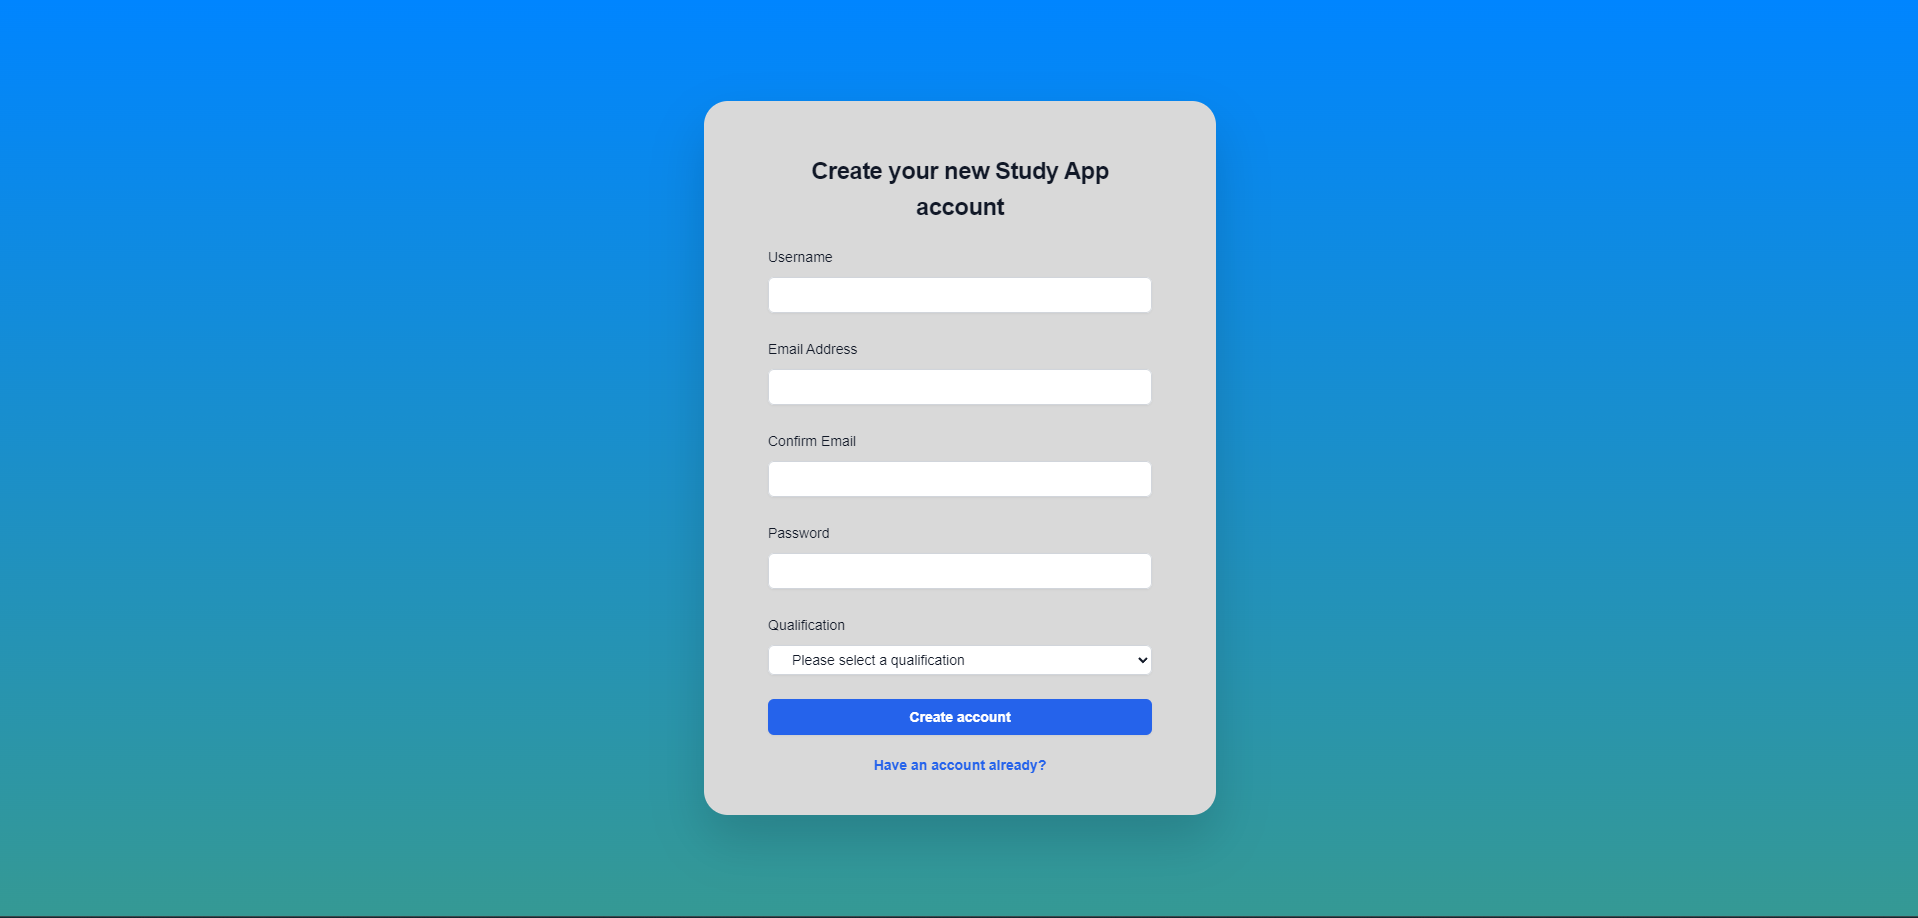
\includegraphics[scale=0.3]{create}
\captionof{figure}{The Account Creation Page}

When submitted, the frontend will check to make sure that the email and email confirmation match. Following that, it also checks if the qualification has a valid input. If neither of these is the case, an alert would show on the screen to inform the user - and nothing would happen.
\\\\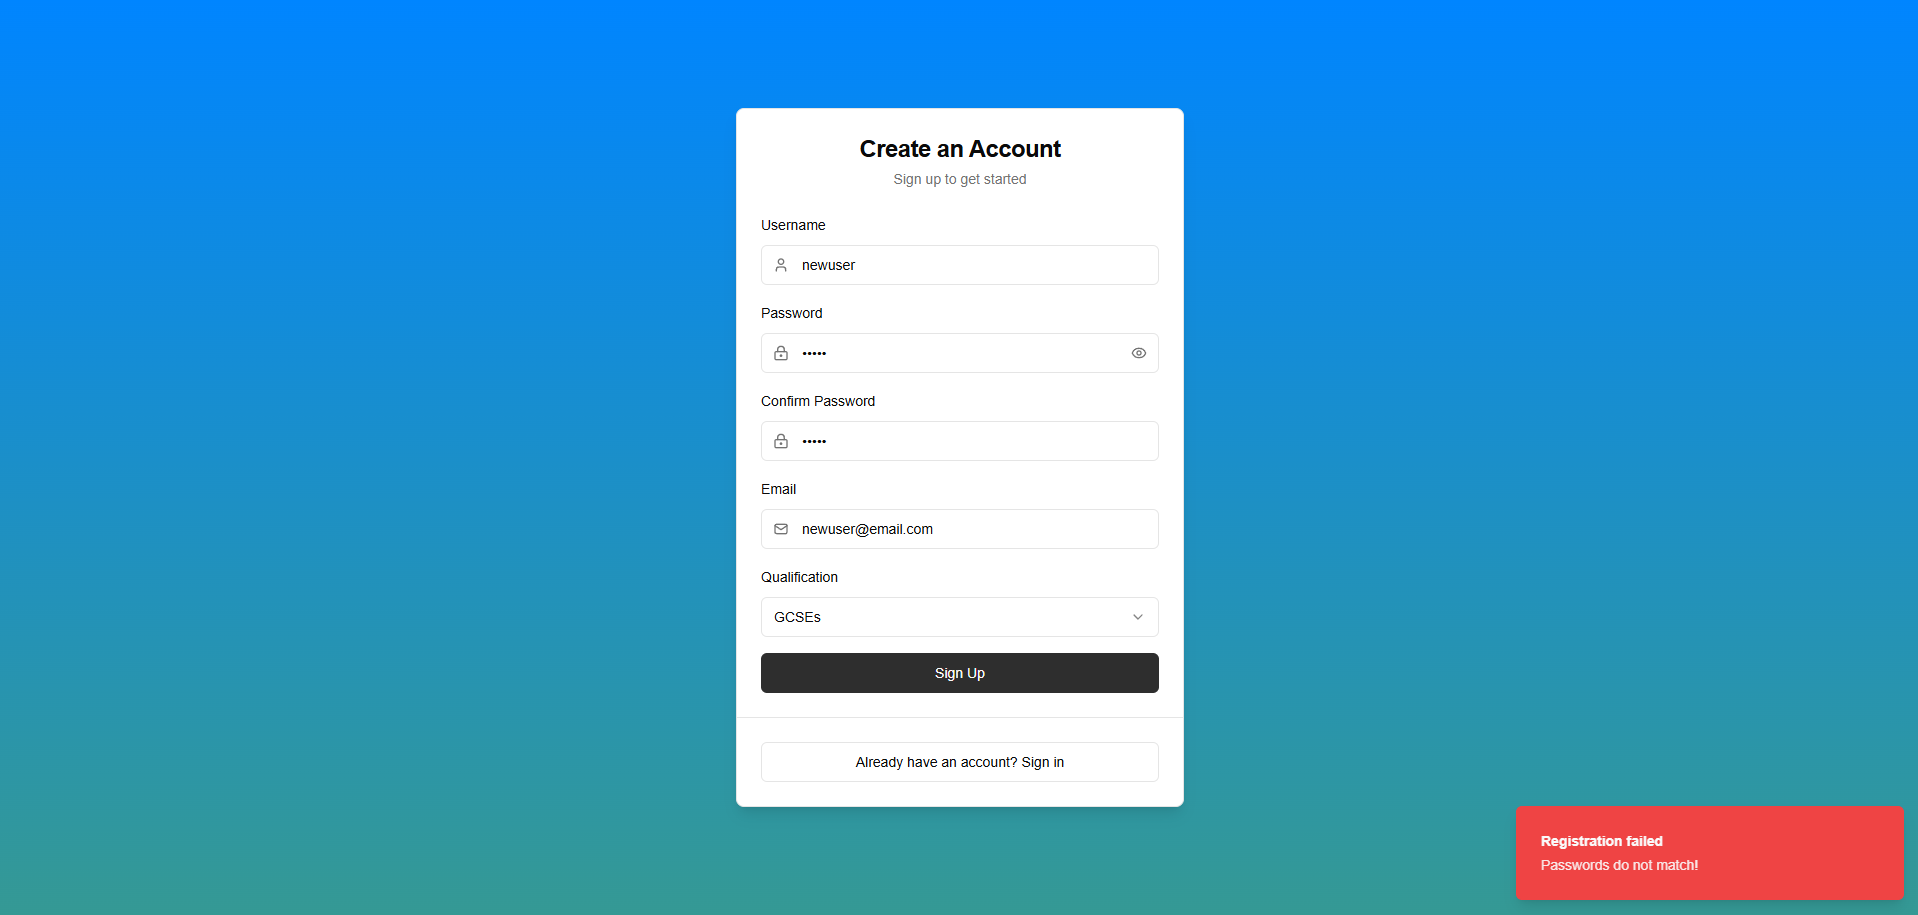
\includegraphics[scale=0.3]{create-alerts}
\captionof{figure}{The alert thrown when the emails do not match.}

\newpage % for formatting
\begin{lstlisting}[language=JavaScript, caption={An excerpt from the frontend code where the conditions are checked for the alerts to be thrown.}]
// create/page.tsx
if (email !== emailConfirm) {
	alert("Please ensure you have entered the correct email address in both sections!");
}
else if (qualificationInput === "") {
	alert("Please select a qualification");
}
\end{lstlisting}

When both of these are satisfied, the frontend will collect the variables together into a JSON body to be submitted with the API POST request to the backend. The frontend then waits for a response from the backend before redirecting the user to the homepage. If any issues were to occur at this stage, an exception would be caught and stop the user from being redirected - instead presenting them with an alert informing them of the error.

\begin{lstlisting}[language=JavaScript, caption={The variables are put together into a JSON array, and are then supplied to axios to be send in a request to the backend. Any exceptions that are thrown are caught and handled appropriately.}]
// create/page.tsx
const payload = {
	"username": username, "email": email, "password": password, "qualification": qualificationInput
}

try {
	const response = await axios.post("http://localhost:8080/api/auth/register", payload);
	alert("Account created successfully.");
	router.push('/login')
	
} catch (error: any) {
	if (error.response && error.response.data) {
		alert(error.response.data || "An error occurred during registration.");
	} else {
		alert("Unable to connect to server.");
	}
}

\end{lstlisting}

\begin{lstlisting}[language=Java, caption={An except from the backend logic creating a User object and saving it to the database.}]
// RegistrationService.java
@Transactional
public User registerUser(RegistrationRequestDto request) throws QualificationException {
	if (userRepository.existsByUsername(request.username()) ||
	userRepository.existsByEmail(request.email())) {
		
		throw new ValidationException(
		"Username or Email already exists");
	}
	
	User user = new User();
	user.setUsername(request.username());
	user.setEmail(request.email());
	user.setPassword(passwordEncoder.encode(request.password()));
	user.setQualificationId(qualificationService.getIdByName(request.qualification()));
	
	return userRepository.save(user);
}
\end{lstlisting}

\section{User Login}
Once the user has created their account, they will be redirected to the login page where they are able to enter their details. Through this, they will be able to access the application to then carry out their revision tasks.
\\\\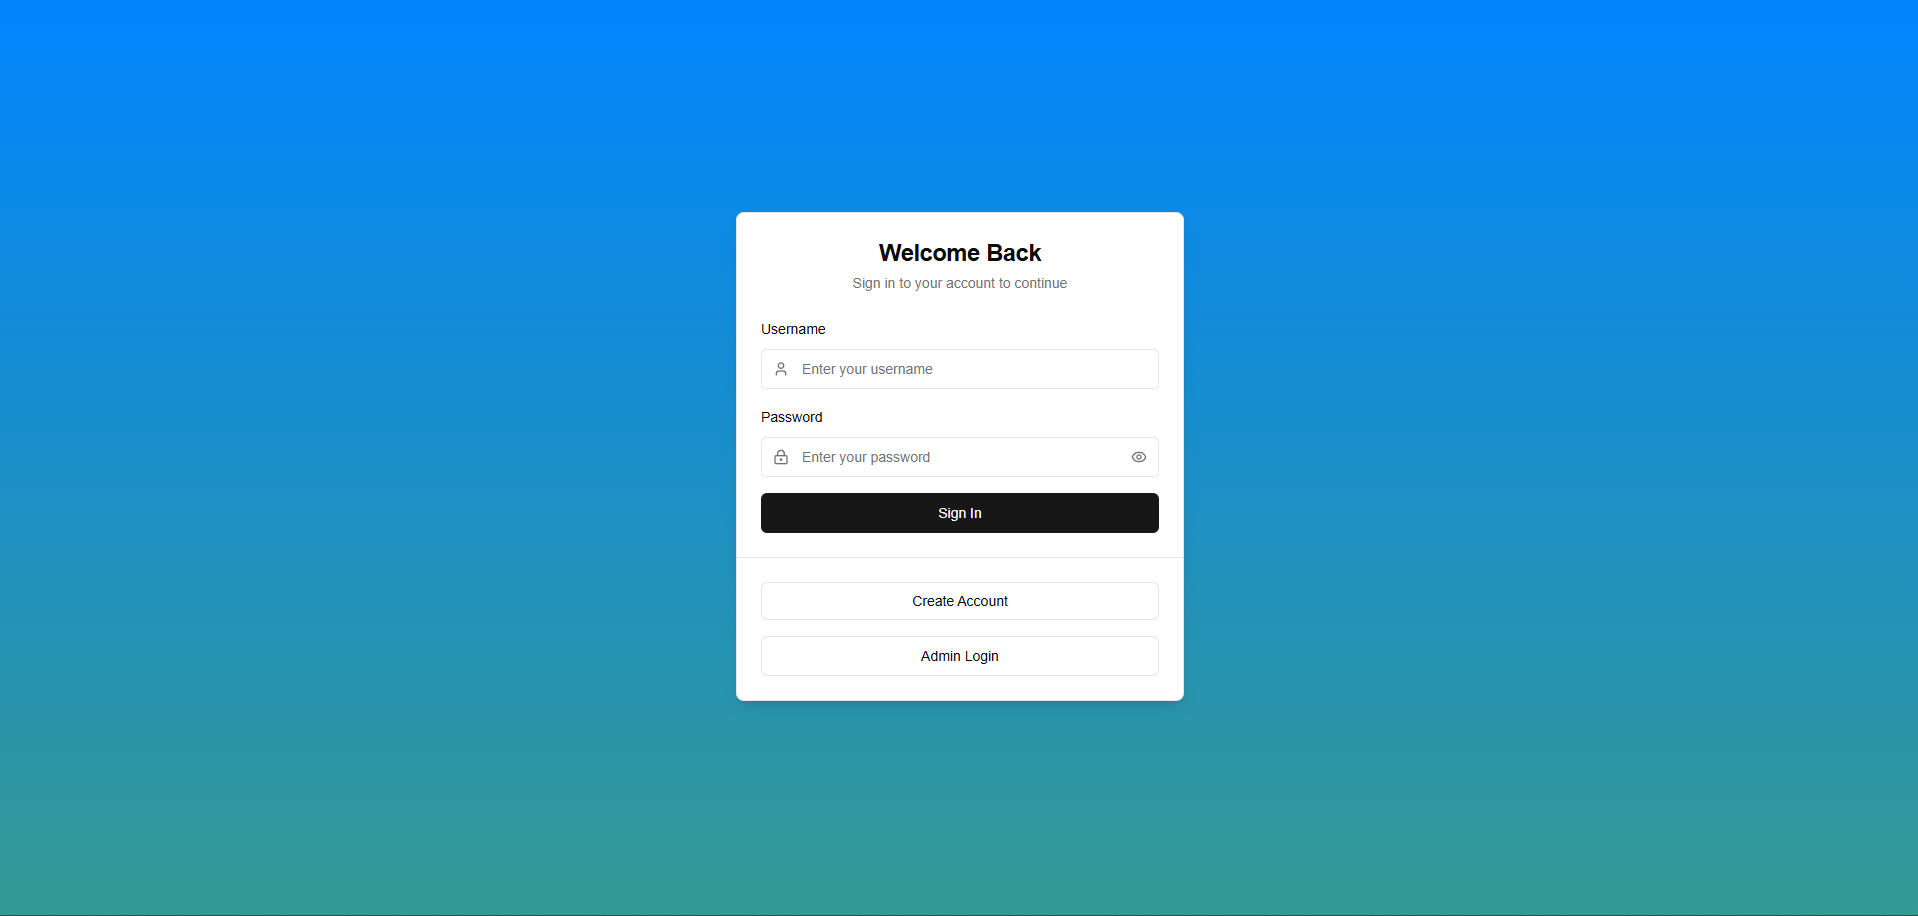
\includegraphics[scale=0.3]{login}

When submitted, the username and password are packaged into a JSON body to be sent via an axios request to the backend. The user details are authenticated, before a JSON Web Token is returned to the frontend as a cookie. This will be used in future API Requests, where the user needs to be authenticated for the functions to be executed. Additionally, a secondary cookie is returned with a timestamp that represents the time two minutes before the token is due to expire. This is used to trigger the refresh token mechanism - so that the token can be automatically refreshed if the user is within the two minute window.

\begin{lstlisting}[language=JavaScript, caption={The username and password are added to a payload, and sent as the request body to the backend}]
// login/page.tsx
const login = async (event: { preventDefault: () => void; }) => {
	event.preventDefault();
	
	const payload = {
		"username": username, "password": password
	}
	
	try {
		const login_confirm = await axios.post("http://localhost:8080/api/auth/login", payload, {withCredentials: true});
		router.push('/dashboard')
		
	} catch (error: any) {
		if (error.response && error.response.data) {
			alert(error.response.data || "An error occurred during logging in.");
		} else {
			alert("Unable to connect to server.");
		}
		
	}
}
\end{lstlisting}

\begin{lstlisting}[language=Java, caption={The controller code showing the steps required to authenticate the user.}]
// AuthController.java
@PostMapping("/login")
public ResponseEntity<String> authenticate(@RequestBody final AuthenticationRequestDto authenticationRequestDto) {
	try {
		AuthenticationResponseDto response = authenticationService.authenticate(authenticationRequestDto);
		ResponseCookie cookie = cookieService.createTokenCookie(response.accessToken());
		ResponseCookie cookieExpire = cookieService.createTimerCookie();
		return ResponseEntity.ok().header(HttpHeaders.SET_COOKIE, cookie.toString(), cookieExpire.toString()).body("User logged in successfully");
	} catch (Exception e) {
		return ResponseEntity.badRequest().body("Username or password is incorrect.");
	}
}
\end{lstlisting}

Both cookies have been designed to be as secure as possible.This includes setting the HTTP-Only and Secure flags to true, so that they are not detected by any external JavaScript - as well as ensuring that the sameSite flag is set to Strict. This way these cookies can only be used within the application itself, and not anywhere else.
\\\\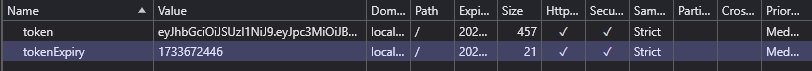
\includegraphics[scale=0.725]{cookies}
\captionof{figure}{Example cookies as they appear in browser's cookies tab.}
\begin{lstlisting}[language=Java, caption={The code used to create the token cookie. For the tokenExpiry the only difference would be the value of the cookie instead.}]
// CookieService.java
public ResponseCookie createTokenCookie(String token) {
	
	return ResponseCookie.from("token", token)
	.httpOnly(true)
	.sameSite("Strict")
	.secure(true)
	.path("/")
	.maxAge(ttl.getSeconds())
	.build();
}

\end{lstlisting}
\section{Refresh Tokens}

The tokens used to verify the user's authenticity have been designed to expire after 15 minutes, for situations where the token is stolen by an attacker.

\section{Dashboard}
Placeholder Text.
\\\\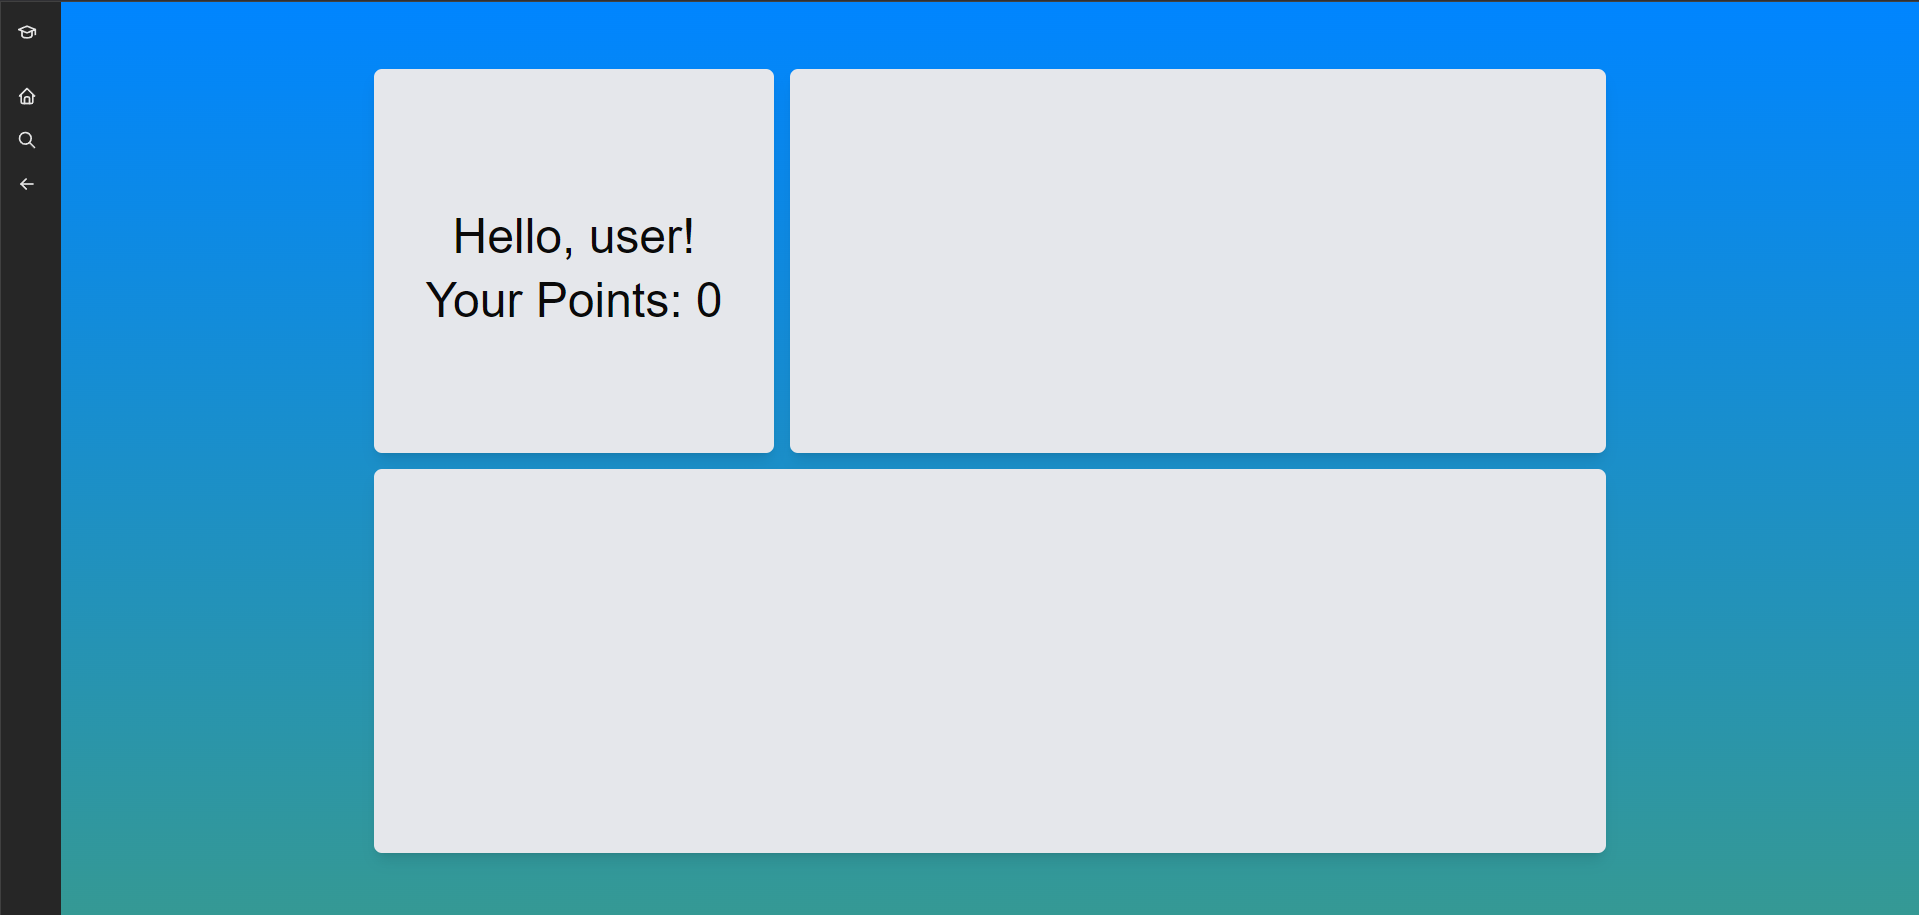
\includegraphics[scale=0.3]{dashboard1}
\\\\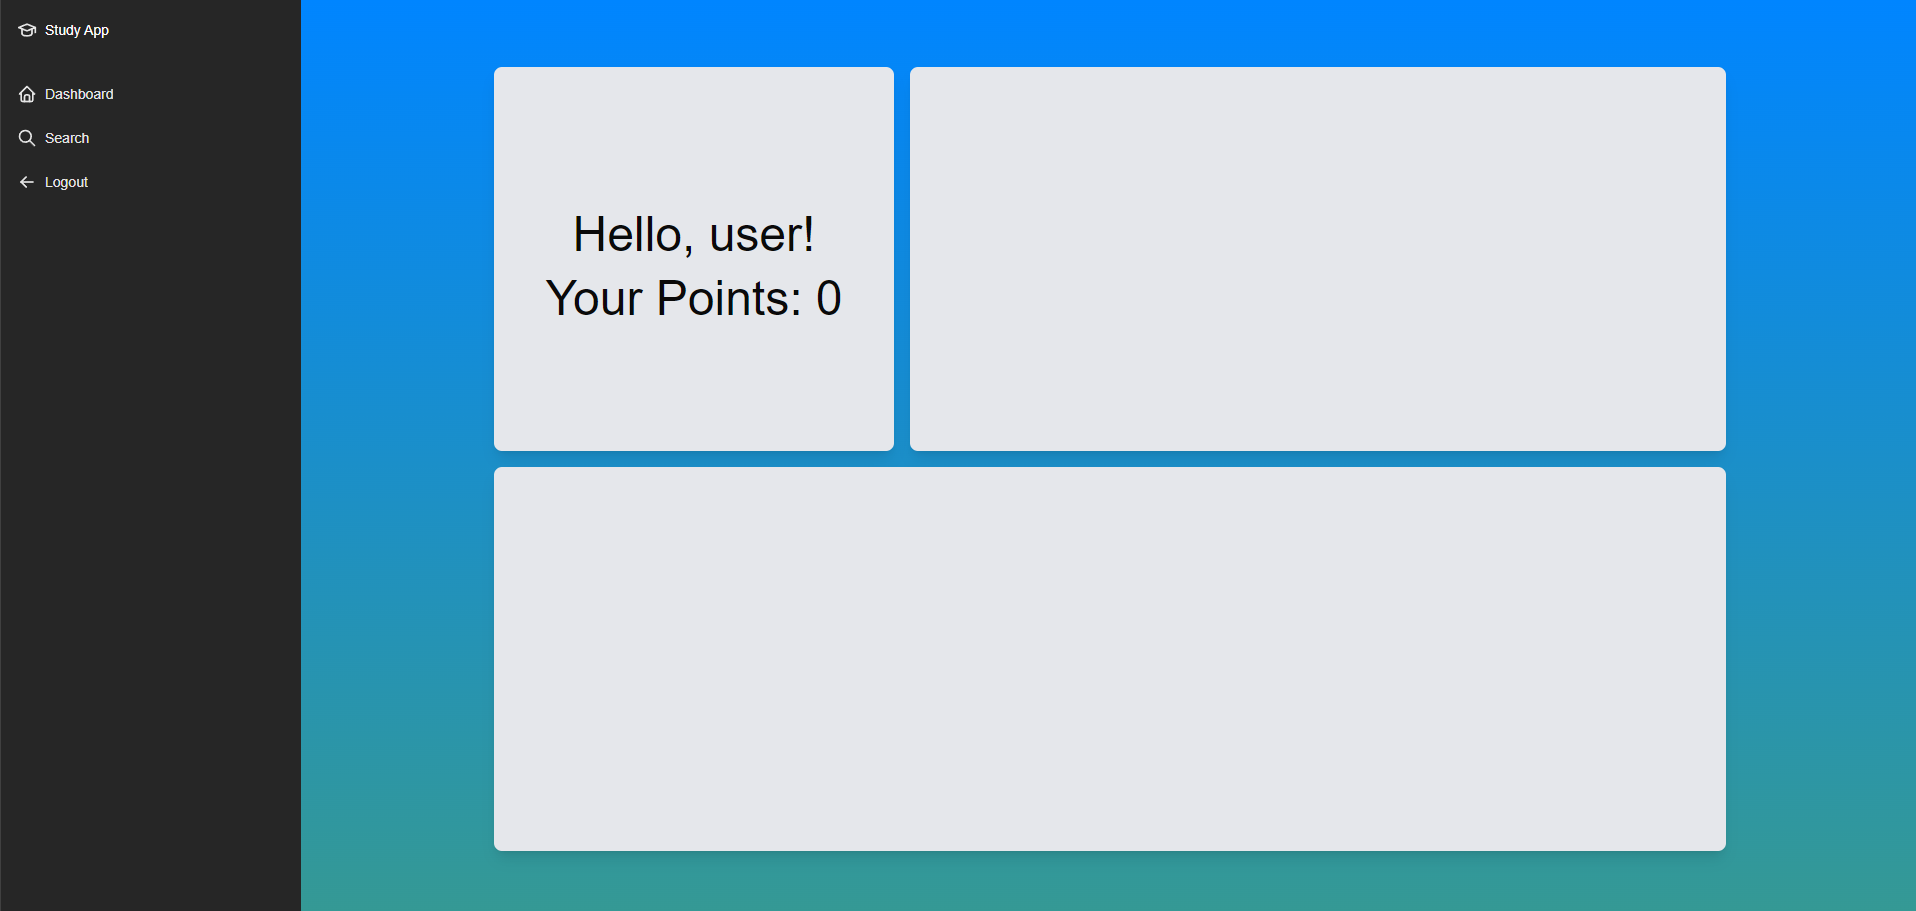
\includegraphics[scale=0.3]{dashboard2}

\section{Subject Search \& Topics}
Placeholder Text.
\\\\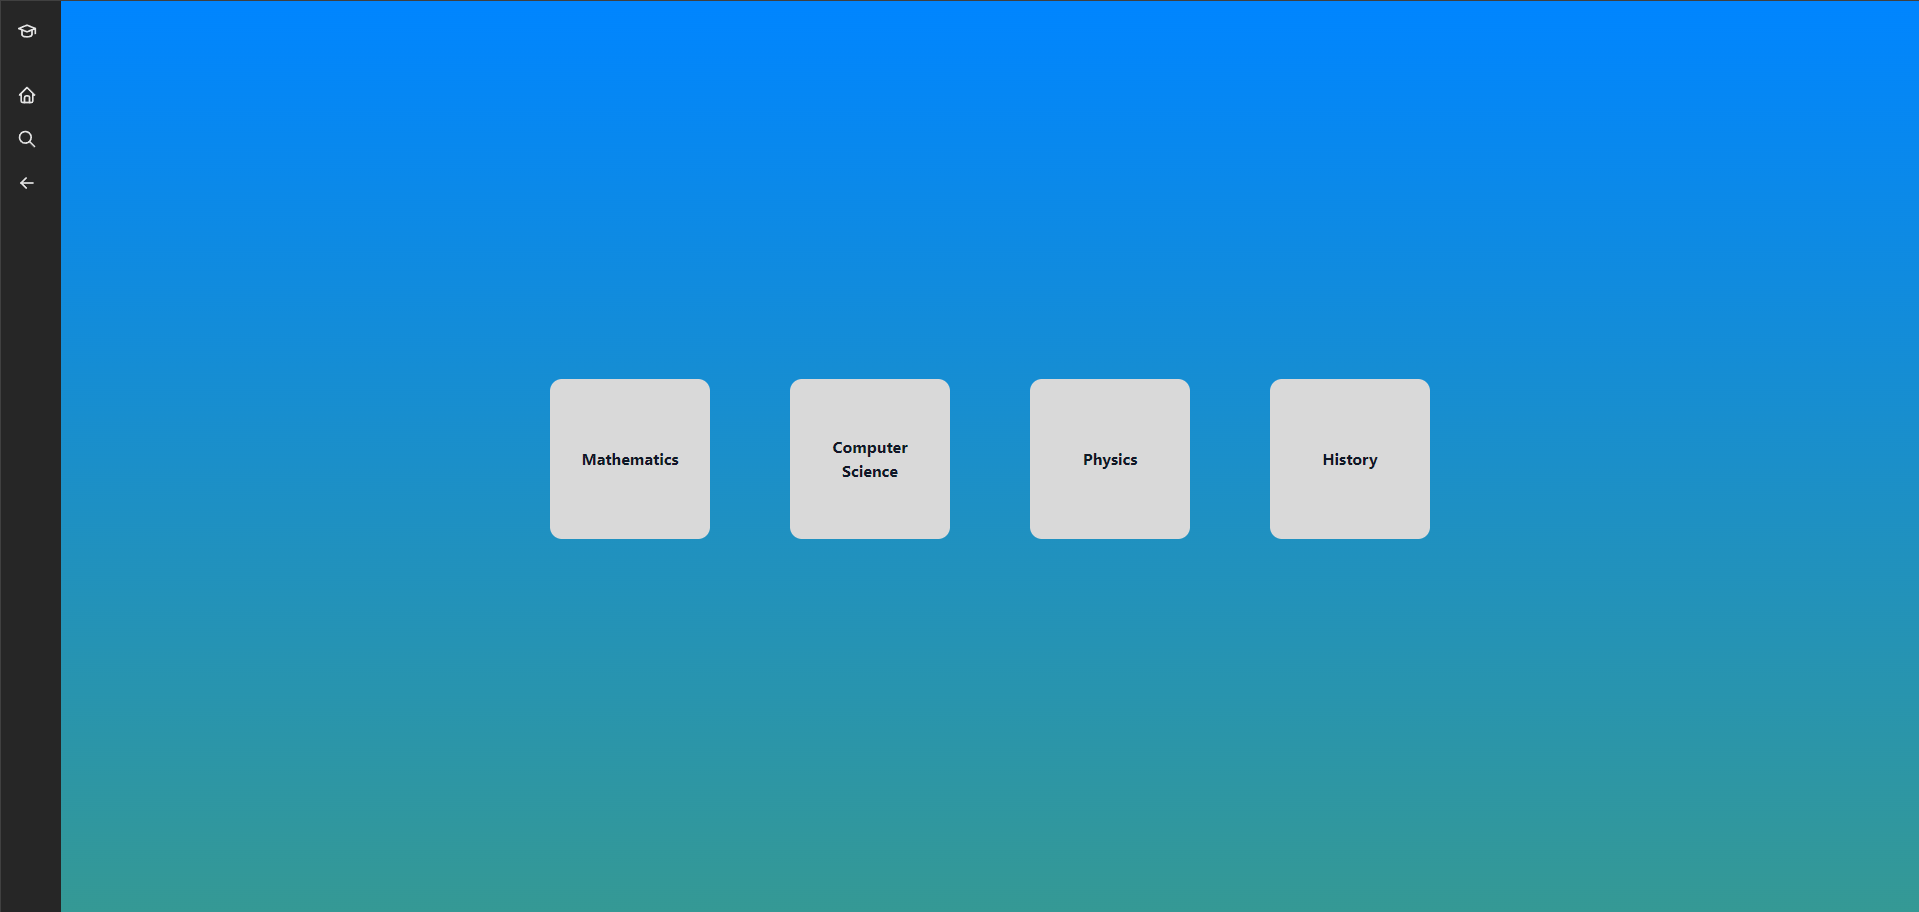
\includegraphics[scale=0.3]{search}
\\\\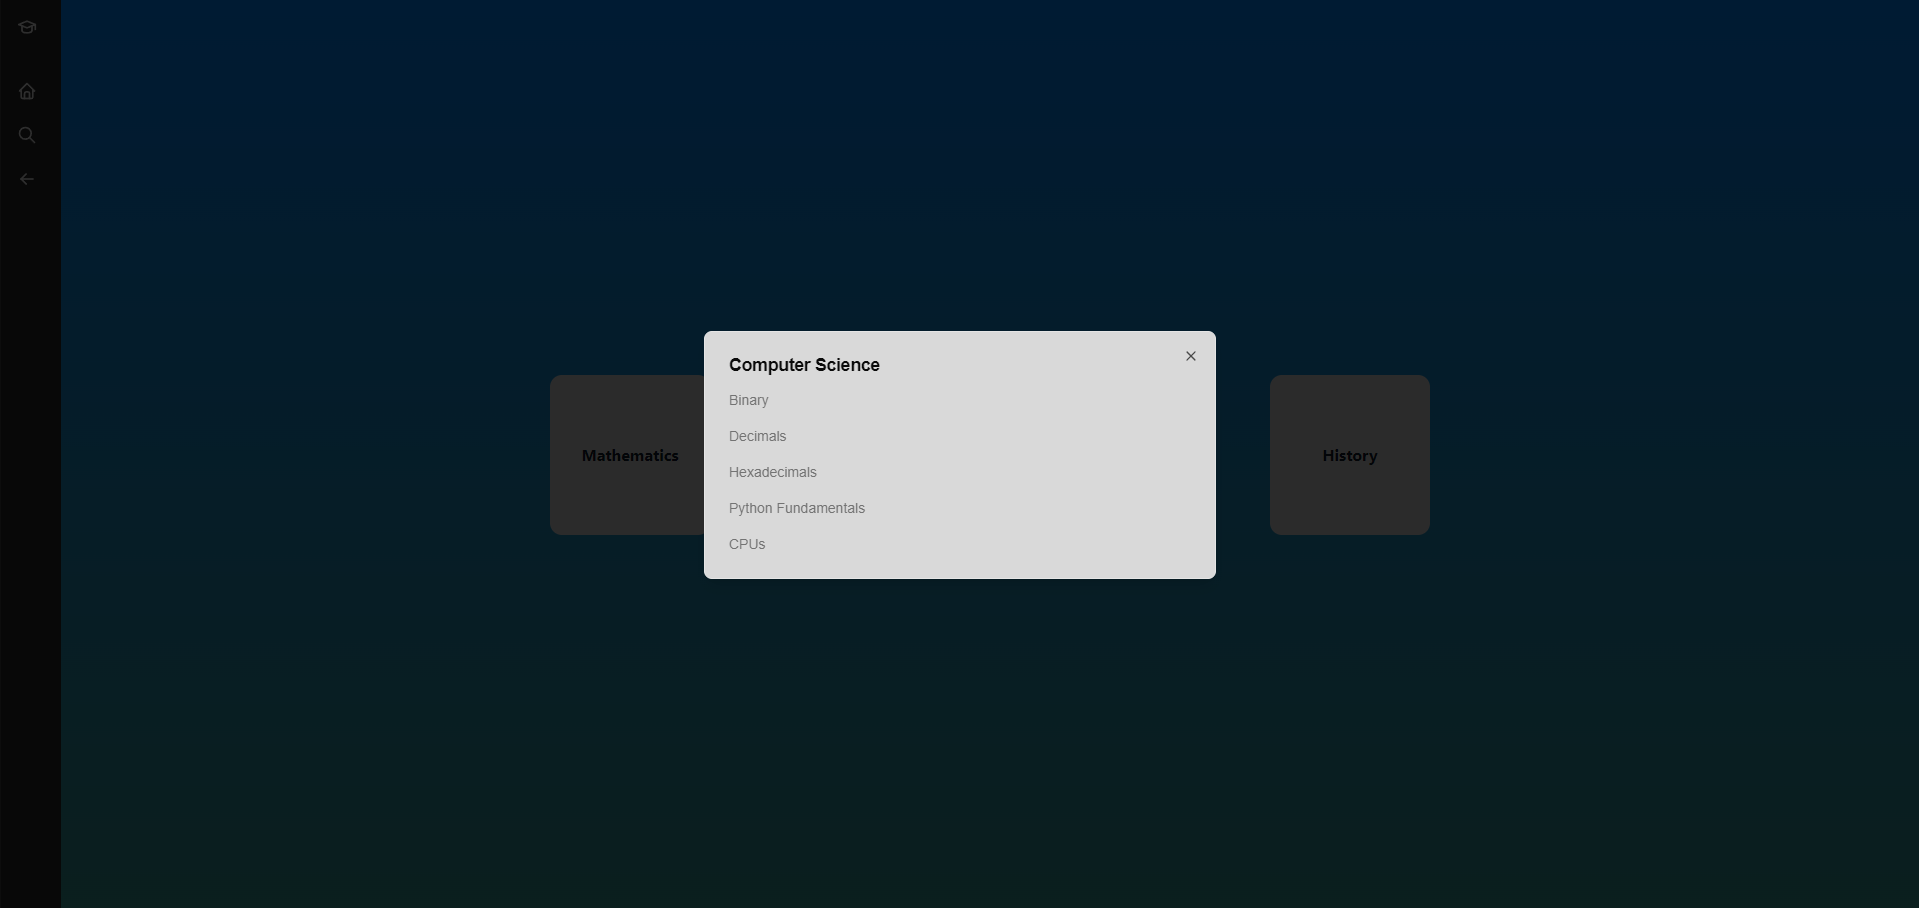
\includegraphics[scale=0.3]{topics}

\chapter{Software Engineering}

\section{Methodology}
\section{Requirements Analysis}
\section{UML Diagrams}
\section{Testing}
\section{Documentation}

\chapter{Reflection}
\section{Milestones \& Challenges Faced}
\section{Next Steps}


\begin{thebibliography}{99}
\addcontentsline{toc}{chapter}{Bibliography}
\bibitem{TBL_WWW} Tim Berners-Lee (1990),
\emph{Information Management: A Proposal - \url{https://www.w3.org/History/1989/proposal.html}}.\\
\textbf{Value:} This is the original proposal document for the World Wide Web, and is where we can how Tim Berners-Lee originally referred to his product as a Universal Linked Information System.

\bibitem{MODERN_WEB} Kyle Brown, Roland Barcia, Karl Bishop, Matthew Perrins (2014),
\emph{Modern Web Development with IBM® WebSphere®: Developing, Deploying, and Managing Mobile and Multi-Platform Apps; Chapter 1 - \url{https://learning.oreilly.com/library/view/modern-web-development/9780133067064/ch01.html}}\\
\textbf{Value:} Provides insight in the history of the Web, and it's evolution to date.

\bibitem{INTERNET_USERS} Ofcom (2023),
\emph{Children and Parents: Media Use and Attitudes, Page 1 - \url{https://www.ofcom.org.uk/siteassets/resources/documents/research-and-data/media-literacy-research/children/childrens-media-use-and-attitudes-2023/childrens-media-use-and-attitudes-report-2023.pdf?v=329412}}.\\
\textbf{Value:} Provides statistical data regarding internet usage, especially those with children - which provides a broad idea of how the internet is widely used in the United Kingdom.

\bibitem{DEVICE_REPORT} Kaspersky (2021),
\emph{Raising the smartphone generation - \url{https://www.kaspersky.com/blog/digital-habits-report-2021/}}\\
\textbf{Value:} Provides a deeper insight on the reasons behind children receiving their own devices, providing an insight in what activities children like to engage with online.


\bibitem{DB_NEXTJS} Dinh Bui (2023),
\emph{Next.JS For Front-End and Compatible Backend Solutions - \url{https://www.theseus.fi/bitstream/handle/10024/800535/Bui_Dinh.pdf?sequence=2}}\\
\textbf{Value:} Goes into detail about the benefits of Next.JS and it's advantages over using React.

\bibitem{SPRING} Yashsonker (2024),
\emph{SpringBoot vs Node.js: Which Backend Framework Should You Learn in 2024? - \url{https://medium.com/@yashsonker1998/springboot-vs-node-js-which-backend-framework-should-you-learn-in-2024-1ed9f643a5d0}}\\
\textbf{Value:} Identifies the two most popular backend frameworks and presents comparisons between the two.

\bibitem{SQL} Raif Deari, Xhemal Zenuni, Jaumin Ajdari, Florije Ismaili, Bujar Raufi (2018),
\emph{Analysis And Comparision of Document-Based Databases with Relational Databases: MongoDB vs MySQL - \url{https://ieeexplore.ieee.org/stamp/stamp.jsp?tp=&arnumber=8510719&tag=1}}\\
\textbf{Value:} Explains the differences between ACID and BASE databases, and the pros and cons of each.


\end{thebibliography}

\chapter*{Appendix}
\addcontentsline{toc}{chapter}{Appendix}
\section*{Diary}
\addcontentsline{toc}{section}{Diary}

\section*{Demo}
\addcontentsline{toc}{section}{Demo}
A demonstration of the application at its current stage can be viewed here: [link]

\end{document}

\end{article}
